\section{Incremental PCA}
\label{sec:intro}

%-------------------------------------------------------------------------
\subsection{Important parameter in implementation: $d_3$}
To implement incremental PCA, we utilized the algorithm from the "Online Learning" slides presented in class. Here, a key parameter is $d_2$ and $d_3$. When new data arrives in incremental PCA, computing the eigenspace model for this subset requires $O(\min(D, N')^3)$ time, where $N'$ is the number of data points in the subset. Additionally, merging this new eigenspace model with the existing data takes $O((d_1 + d_2 + 1)^3)$ time, where $d_1$ is equal to the previously computed eigenspace model's $d_3$ value. Therefore, to enhance time efficiency in incremental PCA, it is essential to keep $d_3$ small, although this results in a time-accuracy tradeoff by dropping less-significant eigenvector information, which is represented by our experiment result \cref{fig:q2-fig5}

\begin{figure}
	\centering
	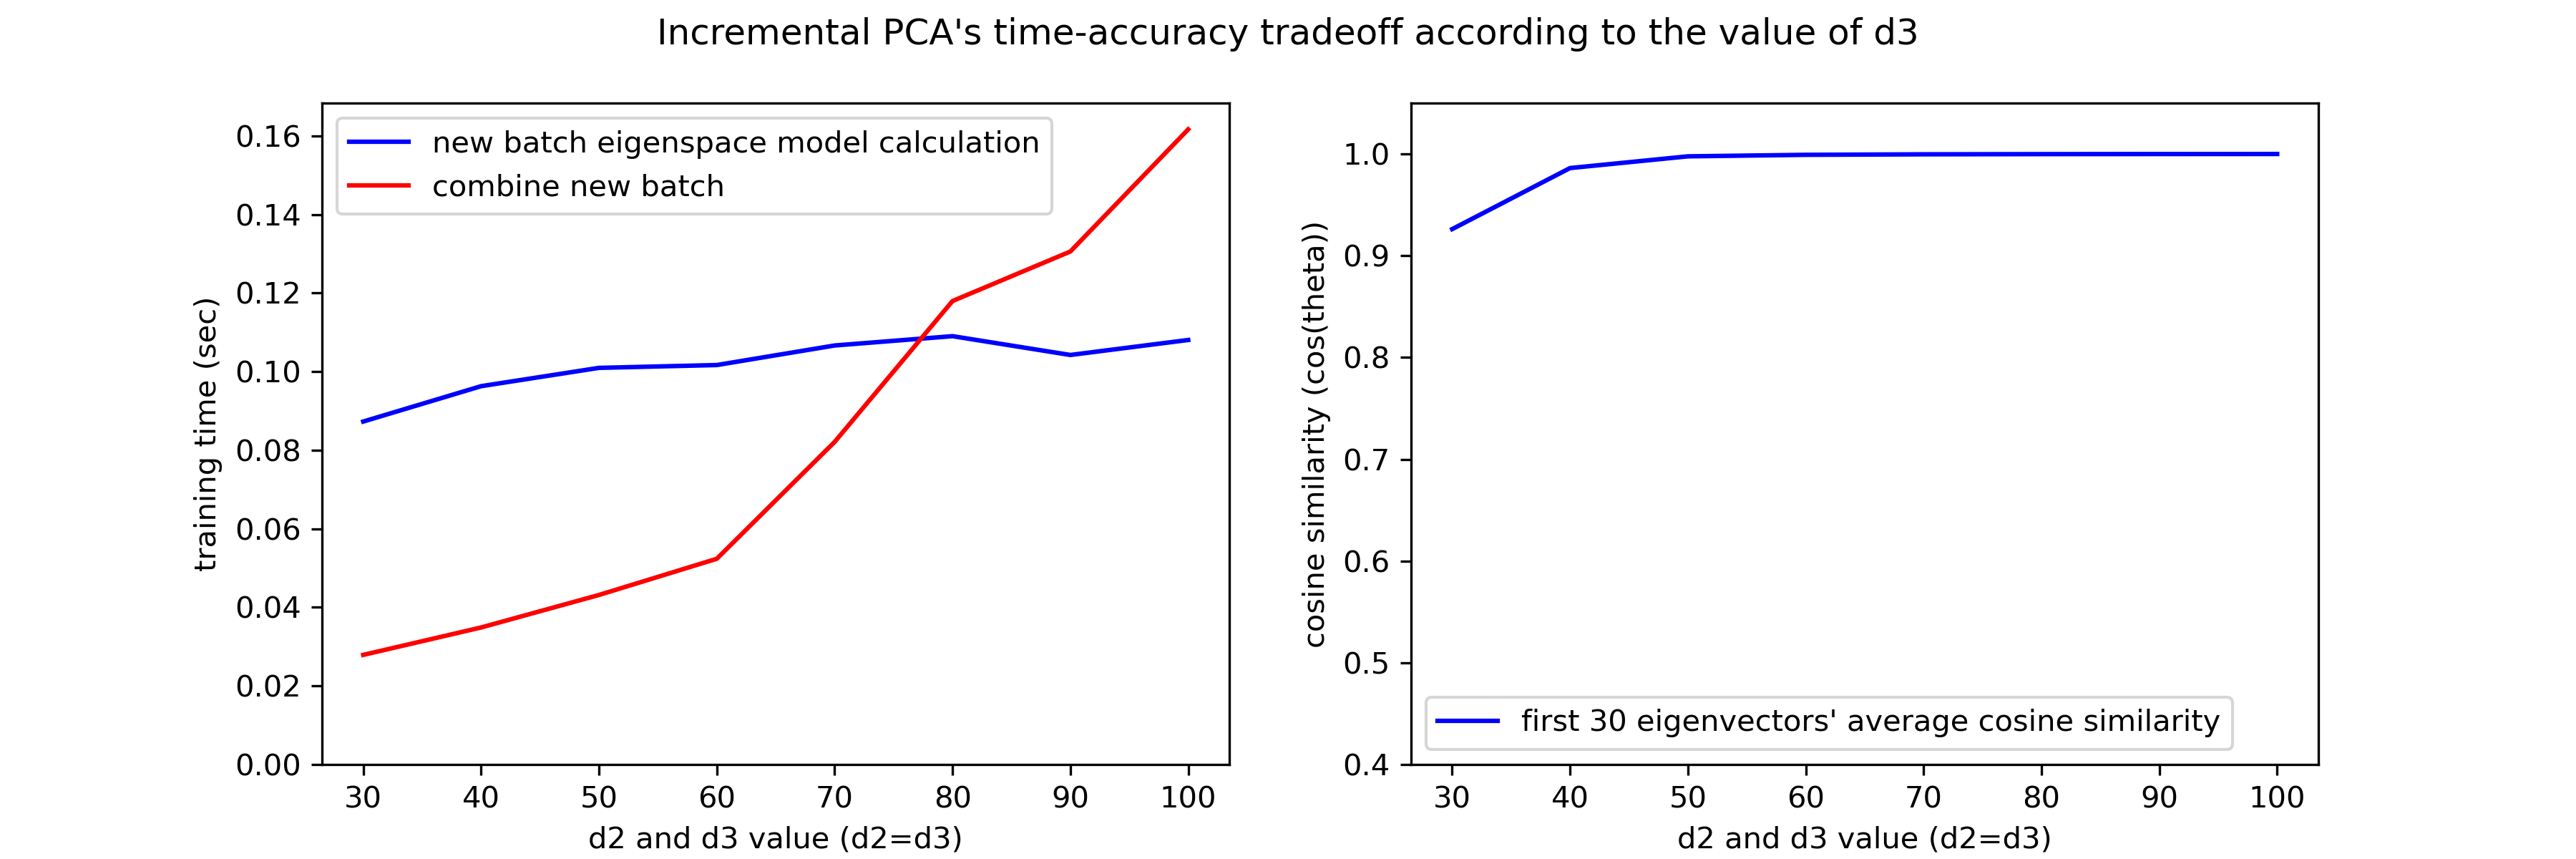
\includegraphics[width=\linewidth]{image/q2-fig5.png}
	
	\caption{Incremental PCA's time-accuracy tradeoff according to the value of $d_3$}
	\label{fig:q2-fig5}
\end{figure}

\subsection{Comparison with other PCA}
We compared the results of each incremental PCA stage (i.e.adding training data in four batches) with the results of batch PCA in the following four aspects. In summary, incremental PCA is a good approximation of batch PCA, and even requires less training time.
\begin{itemize}
	\item Training time: For batch PCA, we measured training time by re-training the model each time new data was added. The results are shown in \cref{fig:q2-fig1}. Using one subset, the training time is approximately the same for both methods. However, as we add more data, the value of $N$ increases for batch PCA, while the values of $N'$ and $d_3$ remain constant for incremental PCA, maintaining constant time and improving time-wise efficiency.
	
	\item Accuracy of incremental PCA: In incremental PCA, time-accuracy tradeoff occurs since less-significant eigenvectors are dropped during $d_1 + d_2$ merging, retaining only the top $d_3$ eigenvectors. We calculated the cosine similarity of eigenvectors, eigenvalues, and mean vectors between incremental PCA at each stage and batch PCA calculated by corresponding data, as shown in \cref{fig:q2-fig2}. As more training data is added, the number of discarded less-significant eigenvectors increases, resulting in decreased similarity between eigenvectors; the similarity after adding the last subset is 0.856. For mean vectors and eigenvalues, cosine similarities are 1 and close to 1 respectively, indicating that the incremental PCA is a good approximation.
	
	\item Reconstruction error: Referring to \cref{fig:q2-fig3}, the reconstruction error for incremental PCA using all training data (i.e., after adding the 4th batch) is almost identical to that of batch PCA with the same amount of data. This also demonstrates that incremental PCA gives similar result to batch PCA.
	
	\item Face recognition accuracy: In the optimal settings of batch PCA found in Question1 (i.e. K=1 and bases=90) the accuracy ranks as follows: full-data batch PCA $>$ full-data incremental PCA $>$ PCA using only the first training set. This indicates that classification accuracy improves progressively with the increase in training data. Additionally, using incremental PCA in place of batch PCA results in an accuracy drop of approximately 6.67\%, also indicating a time-accuracy tradeoff.
	
\end{itemize}

\begin{figure}
	\centering
	\begin{subfigure}{0.48\linewidth}
		\centering
		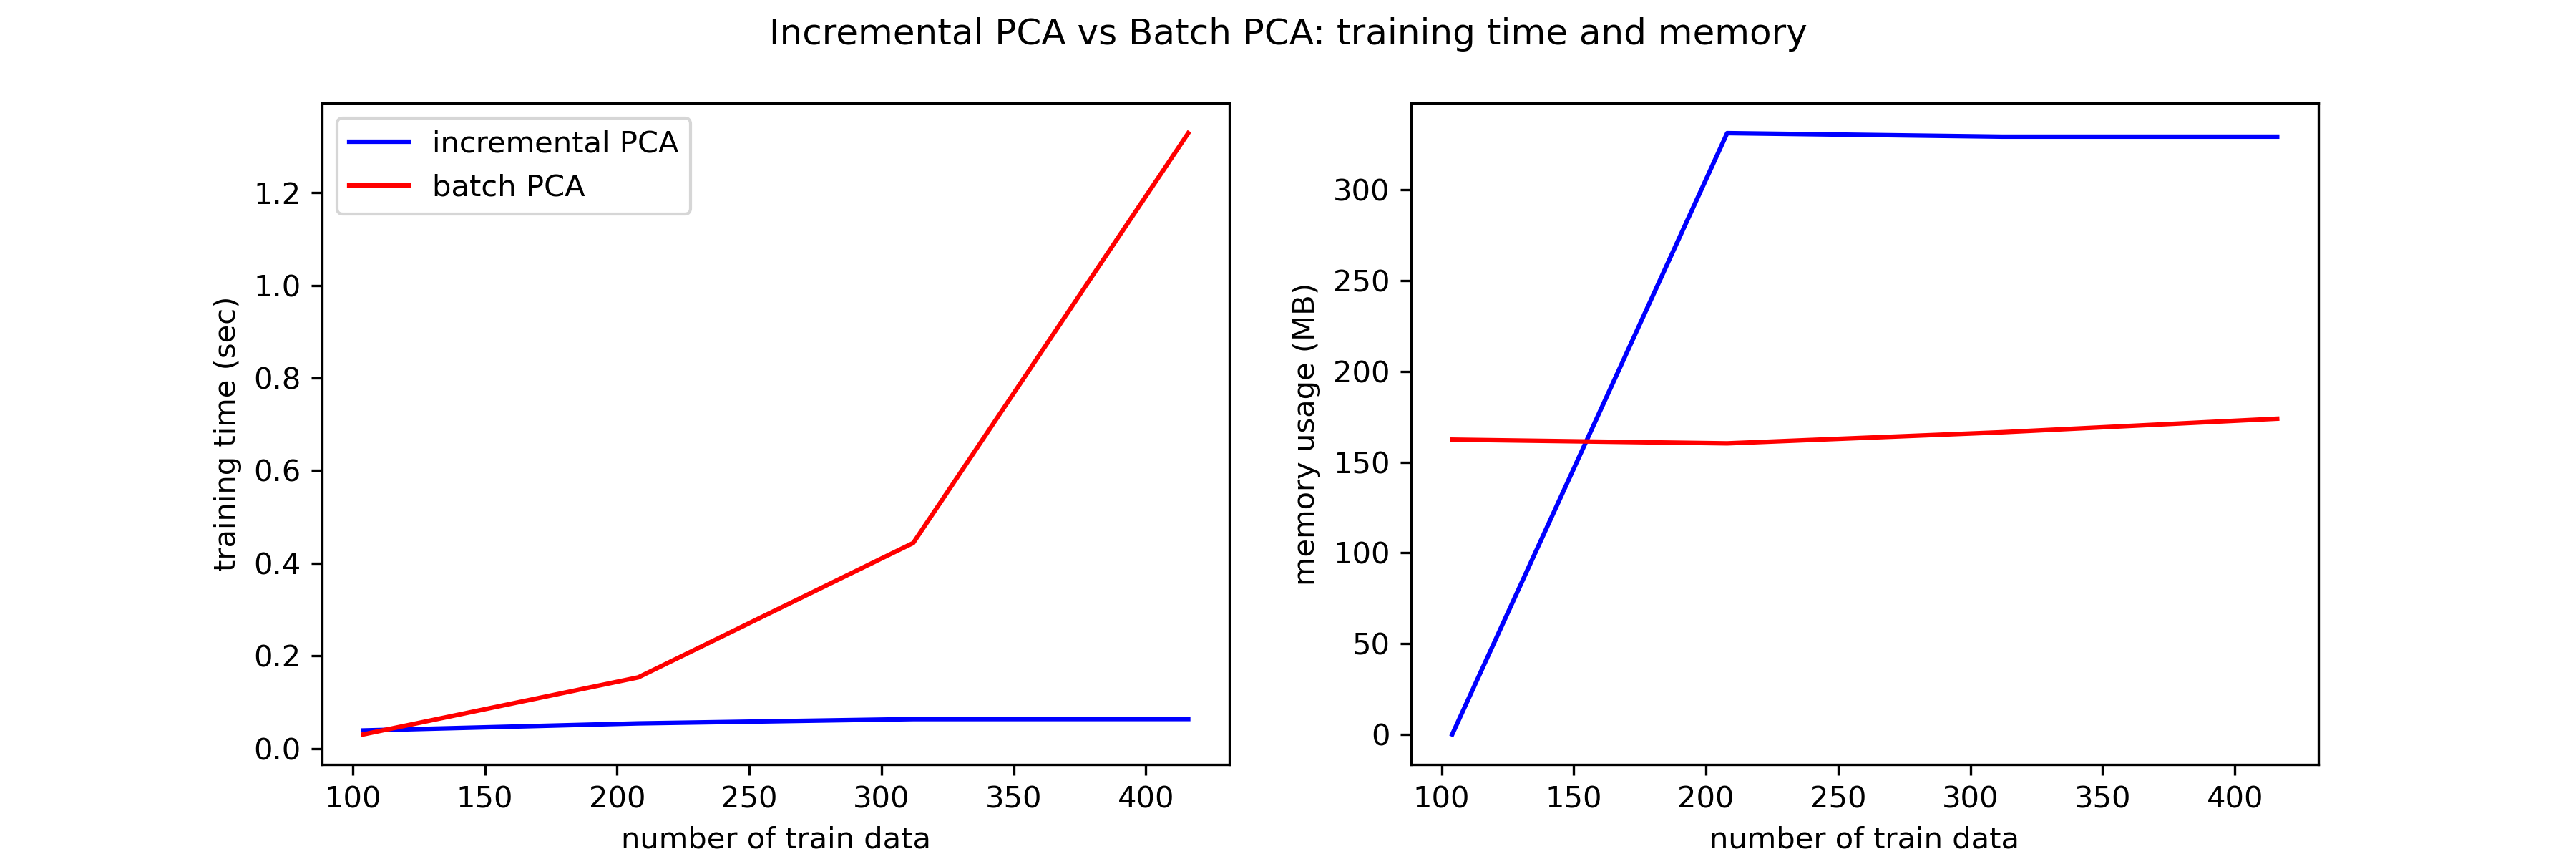
\includegraphics[width=\linewidth]{image/q2-fig1.png}
		\caption{Training time}
		\label{fig:q2-fig1}
	\end{subfigure}%
	\hfill
	\begin{subfigure}{0.48\linewidth}
		\centering
		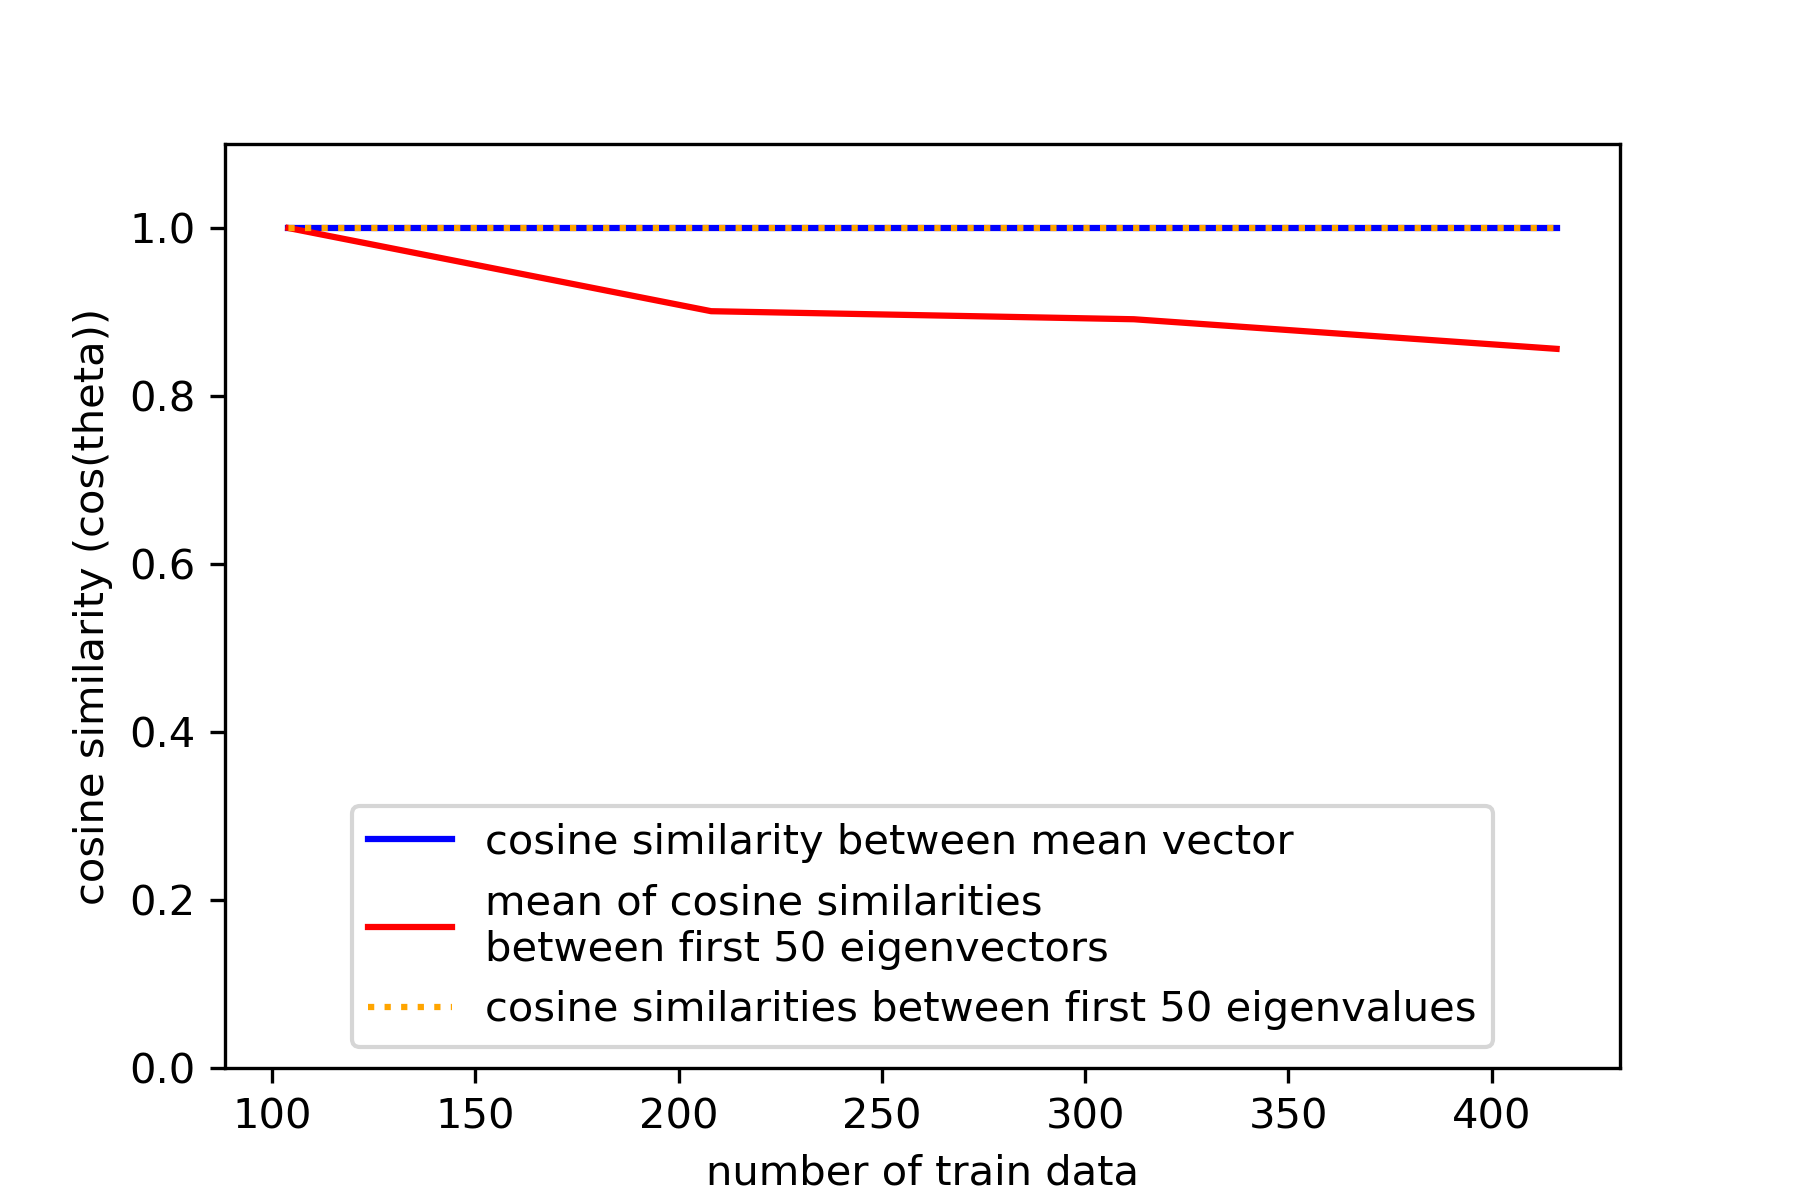
\includegraphics[width=\linewidth]{image/q2-fig2.png}
		\caption{Cosine similarity of results}
		\label{fig:q2-fig2}
	\end{subfigure}
	
	\begin{subfigure}{0.48\linewidth}
		\centering
		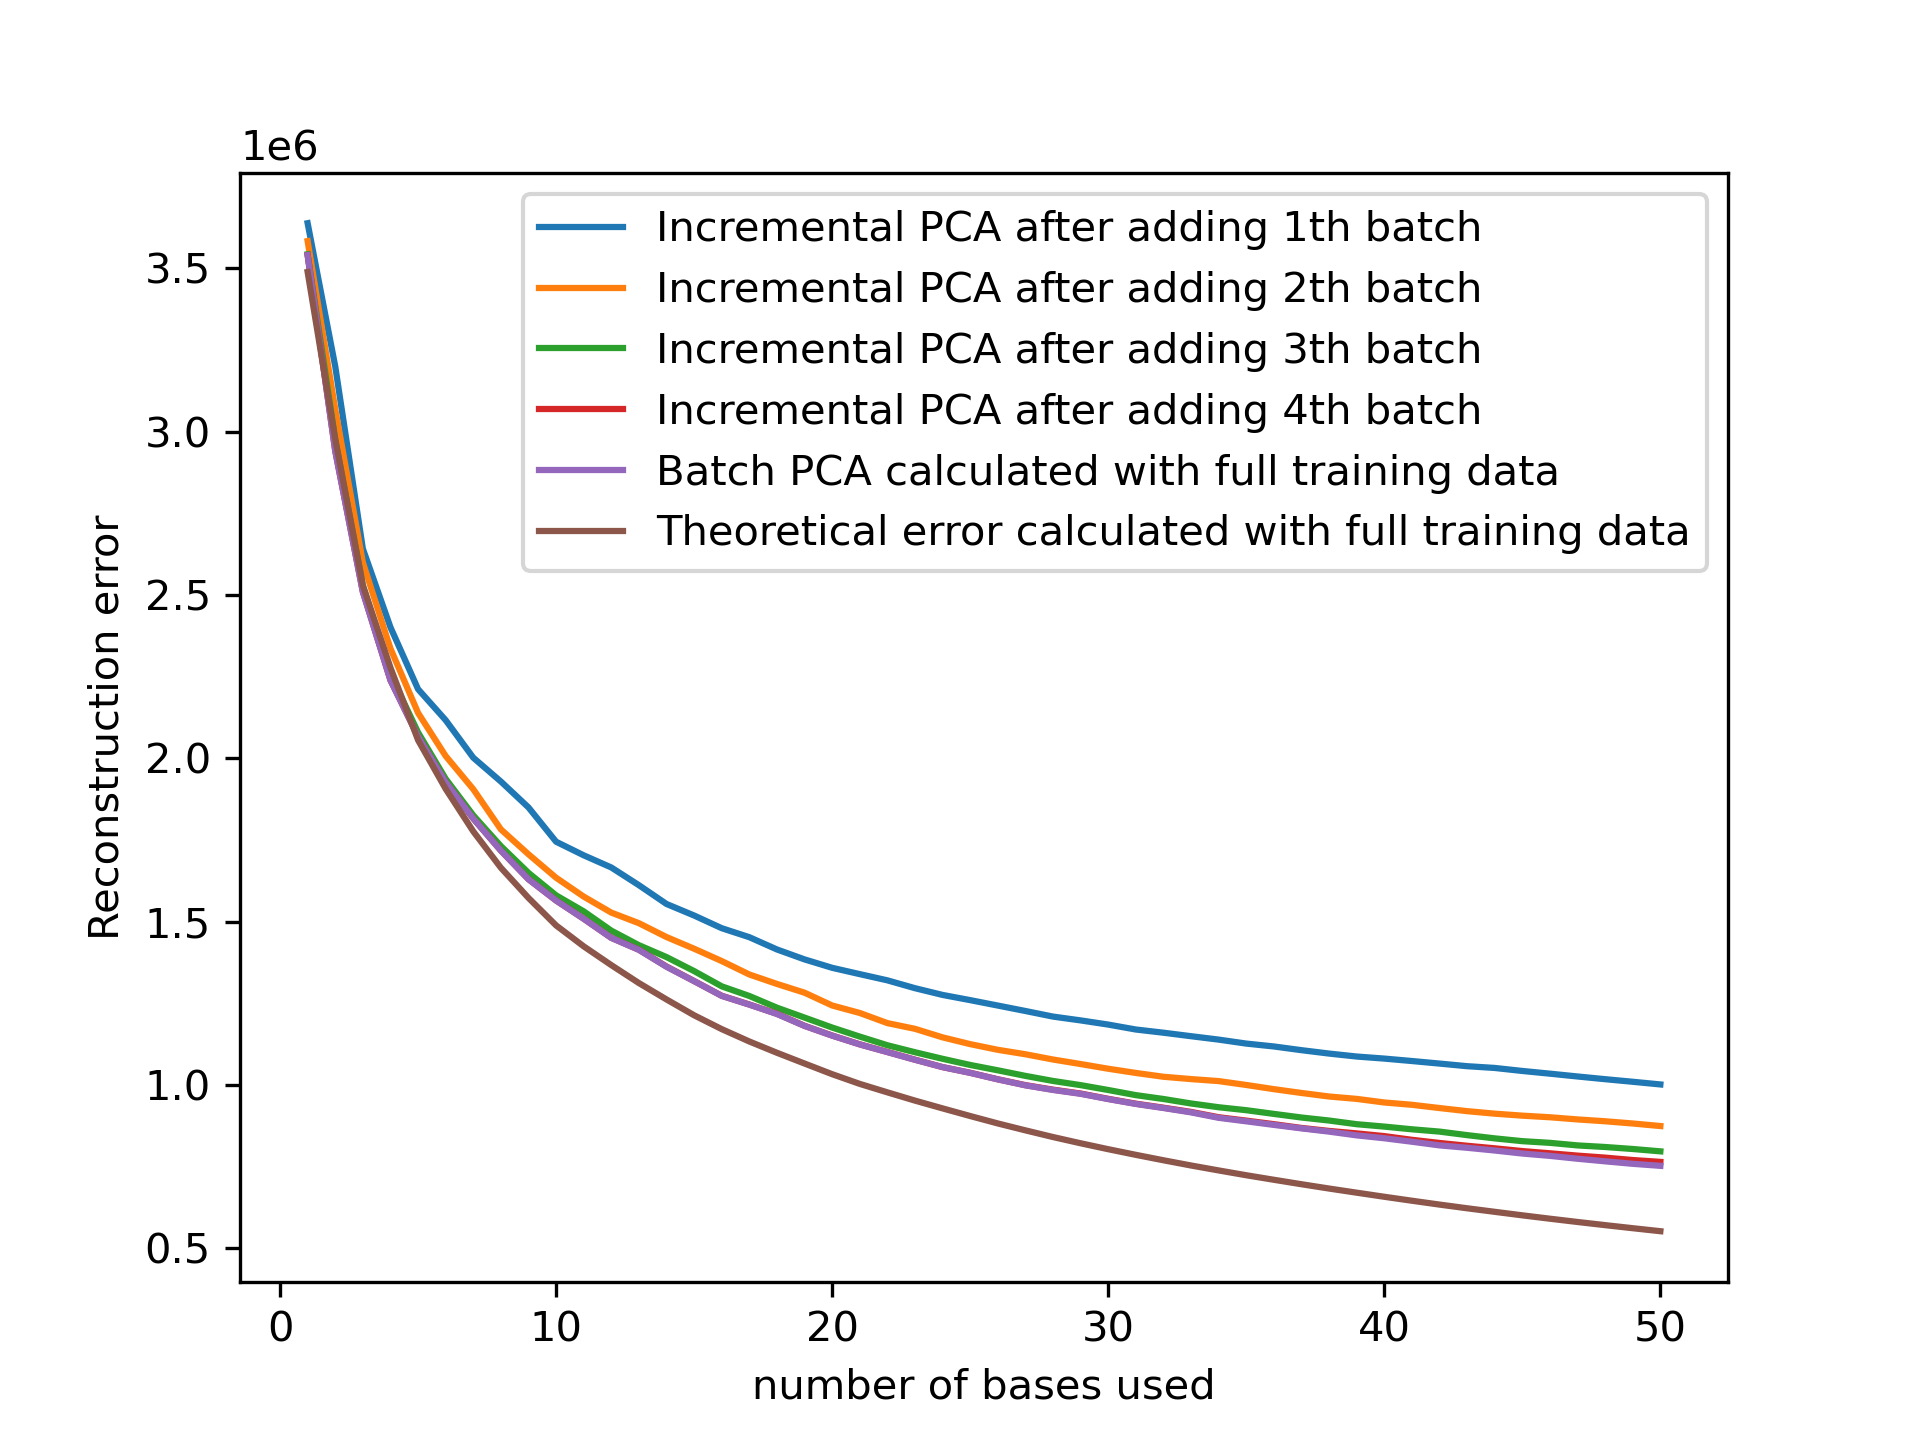
\includegraphics[width=\linewidth]{image/q2-fig3.png}
		\caption{Reconstruction error}
		\label{fig:q2-fig3}
	\end{subfigure}
	\hfill
	\begin{subfigure}{0.48\linewidth}
		\centering
		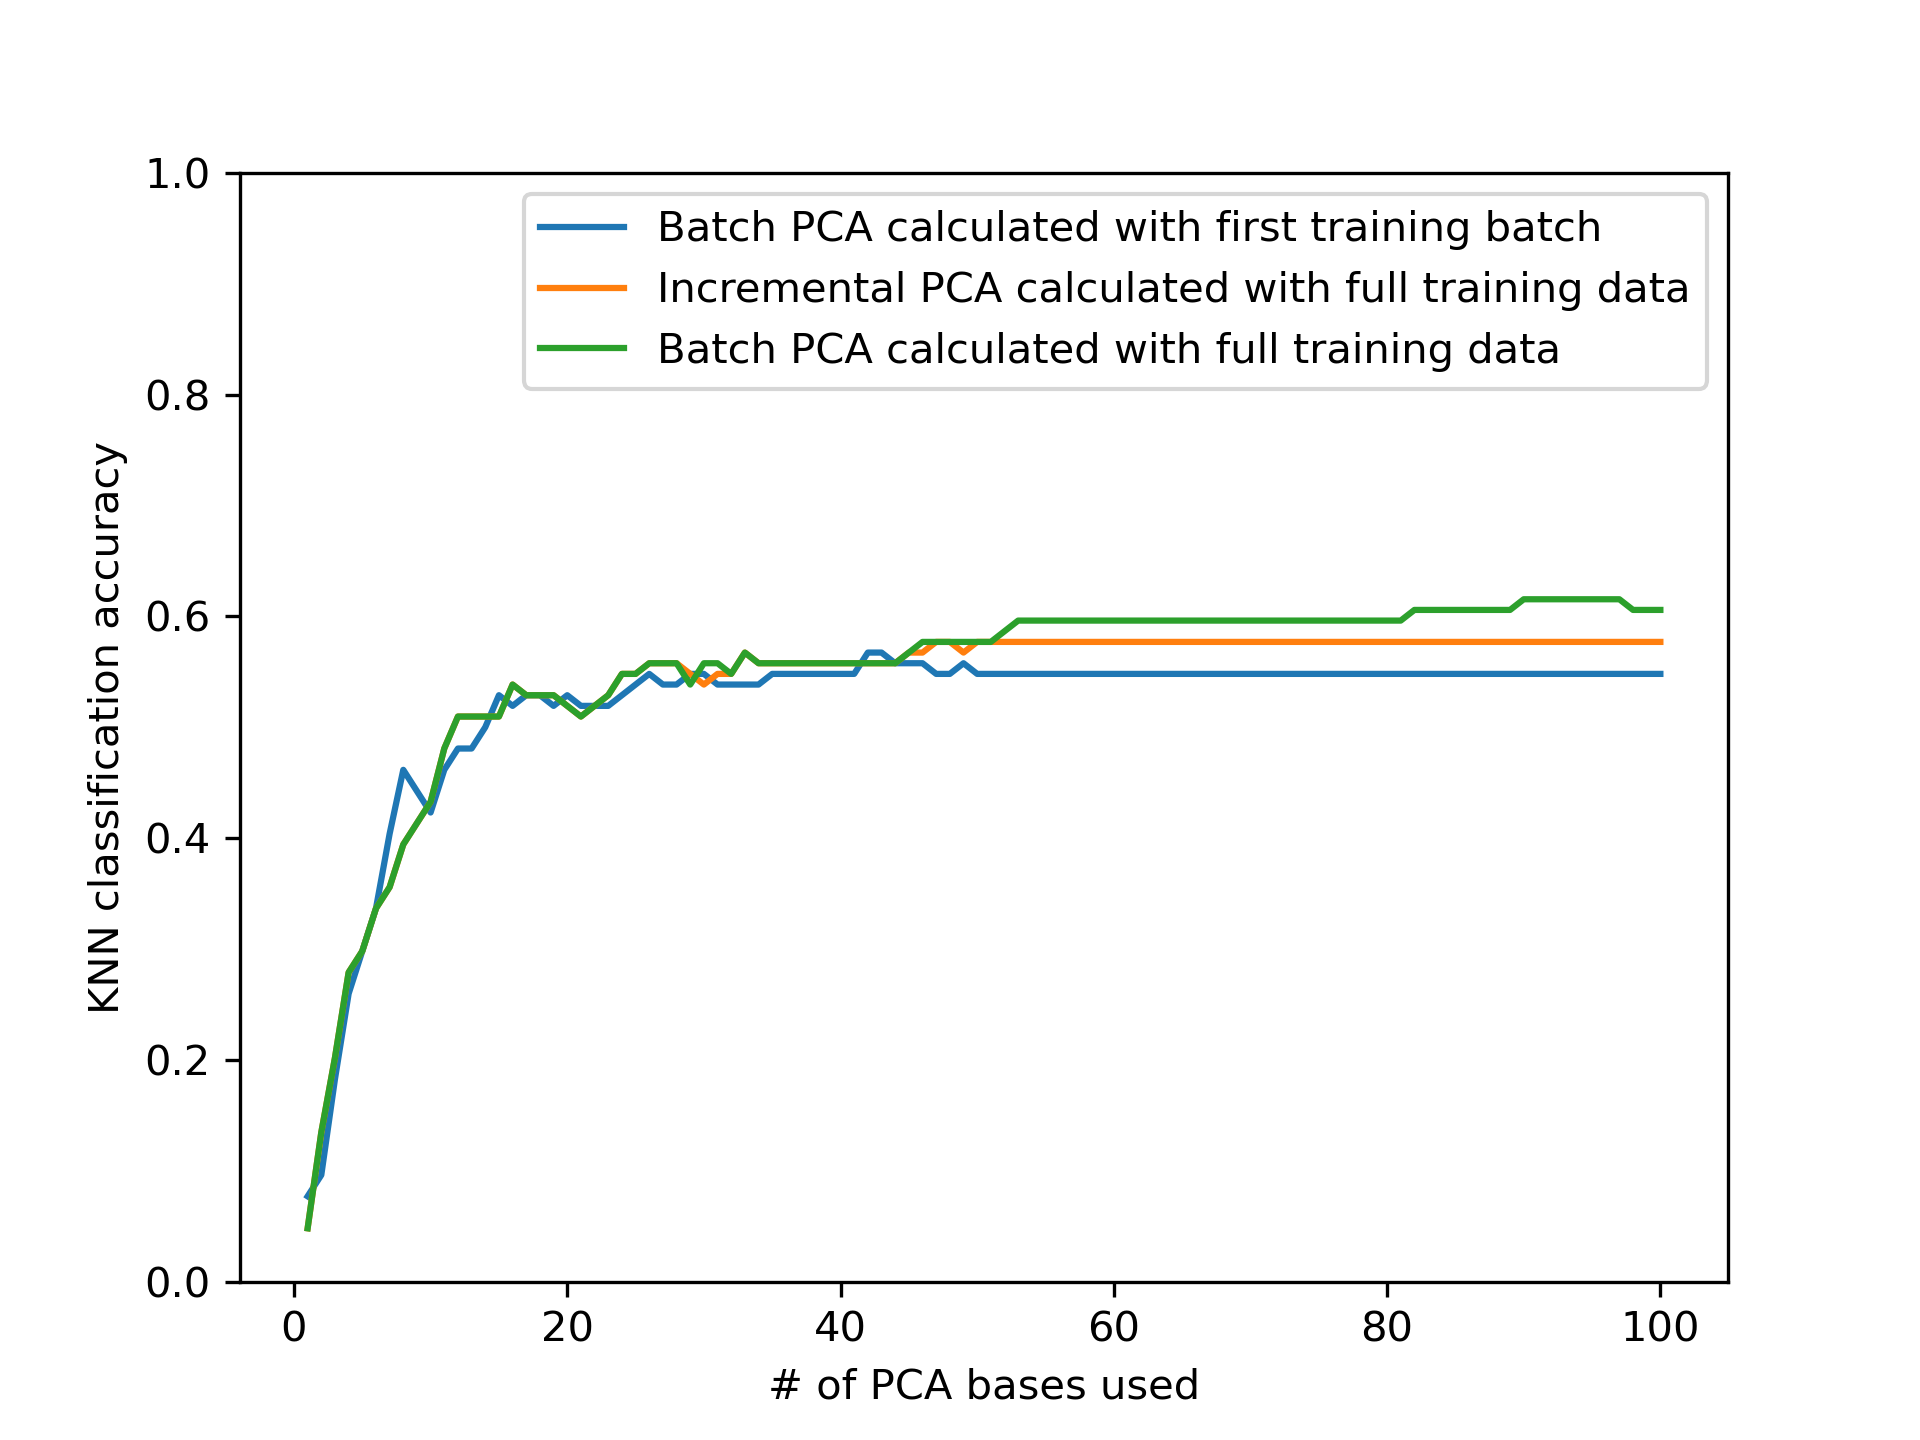
\includegraphics[width=\linewidth]{image/q2-fig4.png}
		\caption{NN-classification face recognition accuracy ($n\_nearest=1$)}
		\label{fig:q2-fig4}
	\end{subfigure}
	\caption{Comparison between Incremental and Batch PCA methods}
	\label{fig:q2}
\end{figure}